\section{Modélisation des systèmes du premier et du deuxième ordre}[Systèmes d'ordre 1 \& 2]
\marginnote[-.5cm]{\xpComp{SLCI}{07}}

\subsection{Systèmes d'ordre 1}


\begin{marginfigure}[3.5cm]
\resizebox{\linewidth}{!}{
\begin{tikzpicture}
\sbEntree{E}
\sbBloc[5]{B1}{$H(p)=\dfrac{K}{1+\tau p}$}{E}
\sbSortie[5]{S}{B1}
\sbRelier[$E(p)$]{E}{B1}
\sbRelier[$S(p)$]{B1}{S}
\end{tikzpicture}}
\end{marginfigure}

\begin{defi}[Système d'ordre 1]
Les systèmes du premier ordre sont régis par une équation différentielle de la
forme suivante :
$$
\tau \dfrac{\dd s(t)}{\dd t}+s(t) = Ke(t).
$$


Dans le domaine de Laplace, la fonction de transfert de ce système est donc
donnée par :

$$
H(p)=\dfrac{S(p)}{E(p)} = \dfrac{K}{1+\tau p}
$$

On note :
\begin{itemize}
 \item $\tau$ la constante de temps en secondes ($\tau>0$);
\item $K$ le gain statique du système ($K>0$).
\end{itemize}
\end{defi}


\begin{marginfigure}
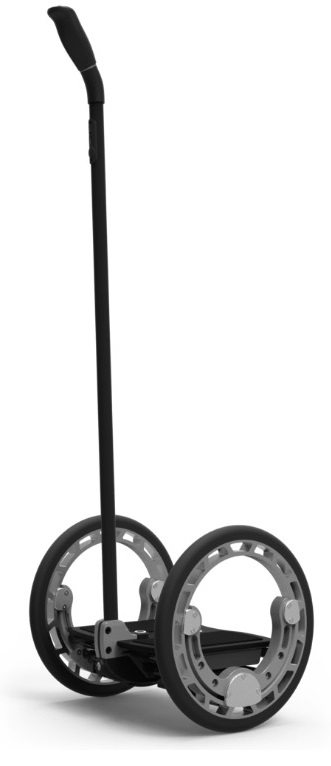
\includegraphics[width=\linewidth]{fig_01}
\end{marginfigure}

\begin{resultat}[Réponse à un échelon d'un système du premier ordre]

On appelle réponse à un échelon, l'expression de la sortie $s$ lorsque on soumet le système à un échelon d'amplitude $E_0$. Lorsque $E_0=1$ ($1/p$ dans le domaine de Laplace) on parle de \textbf{réponse indicielle}.
Ainsi, dans le domaine de Laplace :
$$
S(p)=E(p)H(p) = \dfrac{E_0}{p} \dfrac{K}{1+\tau p}.
$$ 

Analytiquement, on montre que $s(t)=K E_0 u(t) \left(1-e^{-\frac{t}{\tau}}\right)$. 

Si la réponse indicielle d'un système est caractéristique d'un modèle du premier ordre (pente à l'origine non nulle et pas d'oscillation), on détermine :
\begin{itemize}
\item le gain à partir de l'asymptote $K E_0$;
\item la constante de temps à partir de $t_{5\%}$ ou du temps pour $63~\%$ de la valeur finale.% (ou $3\tau$ pour $95~\%$ de la valeur finale).
\end{itemize}
Les caractéristiques de la courbe sont les suivantes : 
\begin{itemize}
\item valeur finale $s_{\infty}=K E_0$;
\item pente à l'origine \textbf{non nulle};
\item $t_{5\%}=3\tau$;
\item pour $t=\tau$, $s(\tau)=0,63~ s_{\infty}$.
%\item Plus $\tau$ est grand, plus le système est lent.
\end{itemize}
\end{resultat}




\begin{marginfigure}
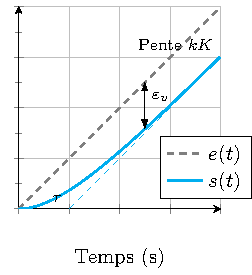
\includegraphics[width=\linewidth]{rampe}
\end{marginfigure}
\begin{resultat}[Réponse à une rampe d'un système du premier ordre]

On appelle réponse à une rampe, l'expression de la sortie $s$ lorsque on soumet le système à une fonction linéaire de pente $k$: 
$$
S(p)=E(p)H(p) = \dfrac{k}{p^2} \dfrac{K}{1+\tau p}.
$$ 


Analytiquement, on montre que $s(t)=Kk \left(t-\tau+\tau e^{-\frac{t}{\tau}}\right)u(t)$. 

Les caractéristiques de la courbe sont les suivantes : 
\begin{itemize}
\item pente de l'asymptote $K k$;
%\item pente à l'origine \textbf{non nulle};
\item intersection de l'asymptote avec l'axe des abscisses : $t=\tau$.
%\item $\varepsilon_{v}=kK\tau$.
%\item Plus $\tau$ est grand, plus le système est lent.
\end{itemize}
\end{resultat}


\subsection{Systèmes d'ordre 2}

\begin{marginfigure}[1cm]
\centering
\begin{tikzpicture}
\sbEntree{E}
\sbBloc[4]{B1}{$\dfrac{K}{1+ \dfrac{2\xi}{\omega_0}p+\dfrac{p^2}{\omega_0^2}}$}{E}
\sbSortie[4]{S}{B1}
\sbRelier[$E(p)$]{E}{B1}
\sbRelier[$S(p)$]{B1}{S}
\end{tikzpicture}
\end{marginfigure}

\begin{defi}[Systèmes d'ordre 2]
Les systèmes du second ordre sont régis par une équation différentielle de la
forme suivante :
$$
\dfrac{1}{\omega_0^2} \dfrac{\dd^2 s(t)}{\dd t^2}+\dfrac{2\xi}{\omega_0} \dfrac{\dd s(t)}{\dd t}+s(t) = Ke(t).
$$

Dans le domaine de Laplace, la fonction de transfert de ce système est donc
donnée par :
$$ H(p)=\dfrac{S(p)}{E(p)} = \dfrac{K}{1+ \dfrac{2\xi}{\omega_0}p+\dfrac{p^2}{\omega_0^2}}. $$

\end{defi}

\begin{itemize}
\item $K$ est appelé le gain statique du système (rapport des unités de $S$ et de $E$);
\item $\xi$ (lire \textit{xi}) est appelé coefficient d'amortissement (sans unité);
\item $\omega_0$ pulsation propre du système ($\text{rad/s}$ ou $s^{-1}$).
\end{itemize}

Suivant la valeur du coefficient d'amortissement, l'allure de la réponse temporelle est différente.





\begin{marginfigure}
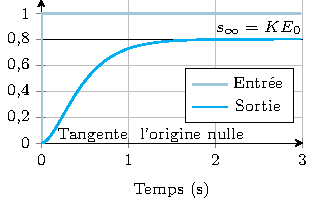
\includegraphics[width=\linewidth]{Ordre2_amorti}
\end{marginfigure}

\begin{resultat}[$\xi \geq 1$ : système non oscillant et amorti \textbf{(apériodique)}]
\begin{itemize} 
\item La fonction de transfert a deux pôles réels.
\item La tangente à l'origine est nulle.
\end{itemize}
\end{resultat}



\begin{marginfigure}
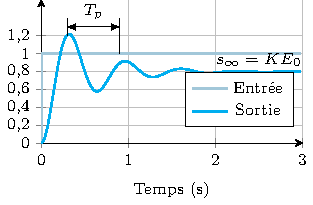
\includegraphics[width=\linewidth]{Ordre2_pseudo}
\end{marginfigure}
\marginnote{Sur la figure ci dessus, le dépassement est de 0,4 et le dépassement pour cent est $D_{\%} = \dfrac{ 0,4}{0,8} = 0,5$.  En utilisant la formule donnée pour identifier $\xi$, on a alors $\xi \simeq 0,15$.}

\begin{resultat}[$\xi <1$ : système oscillant et amorti (pseudo périodique)]
\begin{itemize} 
\item La fonction de transfert a deux pôles complexes.
\item La tangente à l'origine est nulle.
\item La pseudo-période est de la forme $T_p=\dfrac{2\pi }{\omega_0 \sqrt{1-\xi^2}}$.
\item La valeur du premier dépassement vaut :  $D_1=KE_0e^{\dfrac{-\pi \xi }{\sqrt{1-\xi^2}}}$.
\begin{itemize}
\item En notant $D_{\%} =\dfrac{D_1}{KE_0}$, on pourra aussi retenir que $\xi = \sqrt{\dfrac{(\ln D_{\%})^2}{\pi^2 + (\ln D_{\%})^2}}$.
\end{itemize}
\end{itemize}
\end{resultat}

\begin{resultat}
\begin{itemize}
\item Pour $\xi=0$ le système n'est pas amorti (oscillateur harmonique) la réponse à un échelon est une sinusoïde d'amplitude $KE_0$ ($2KE_0$ crête à crête).  
\item Pour $\xi\simeq 0,69$  on obtient le système du second ordre le plus rapide \textbf{avec dépassement}. 
Le temps de réponse à 5\% est donné par $t_{r 5\%} \cdot \omega_0 \simeq 3$.
\item Pour $\xi =1$ on obtient le système du second ordre le plus rapide \textbf{sans dépassement}.

\end{itemize}
\end{resultat}


\begin{figure}
\centering
\begin{subfigure}{0.49\textwidth}
    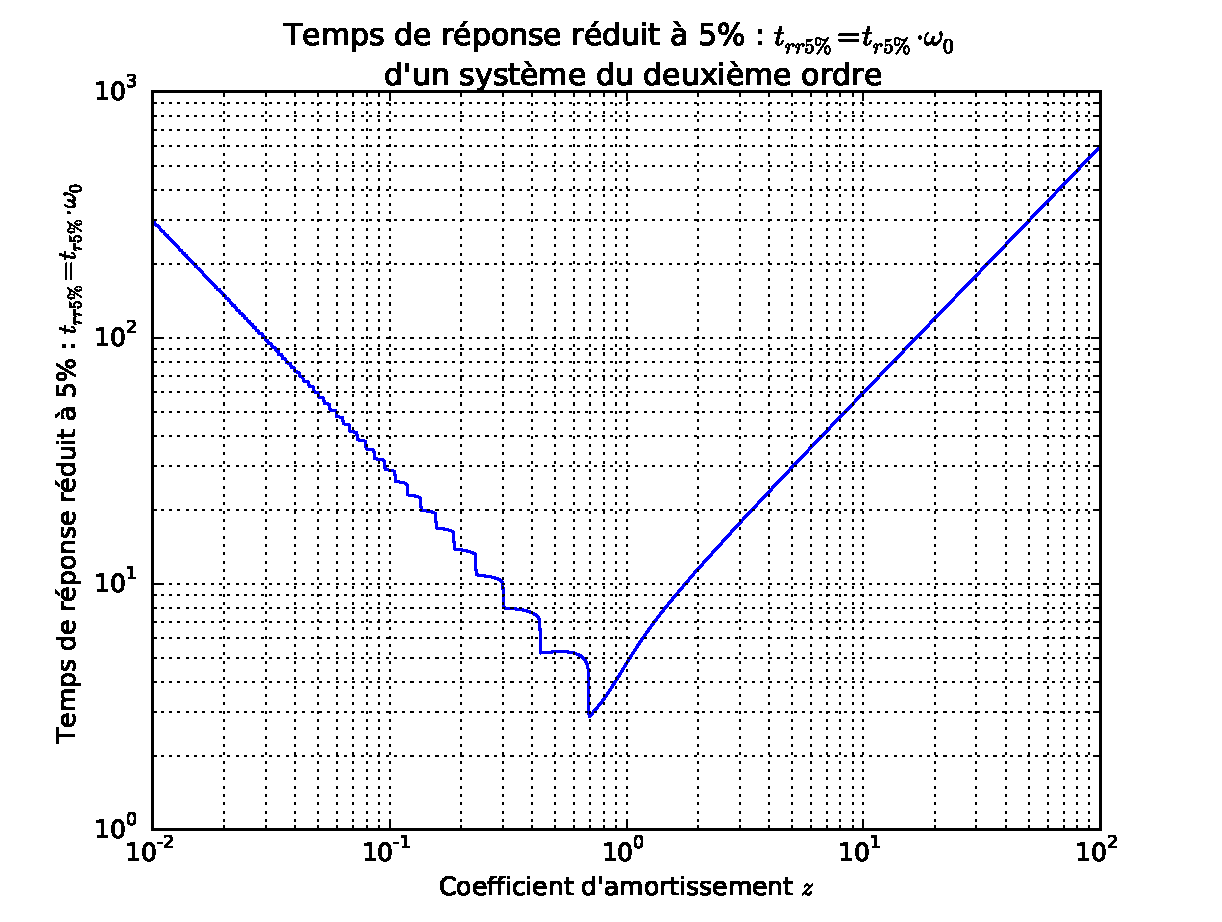
\includegraphics[width=\textwidth]{trr5}
    \caption{Abaque des temps de réponses réduits à 5\, \%}
    \label{fig:t5}
\end{subfigure}
\hfill
\begin{subfigure}{0.49\textwidth}
    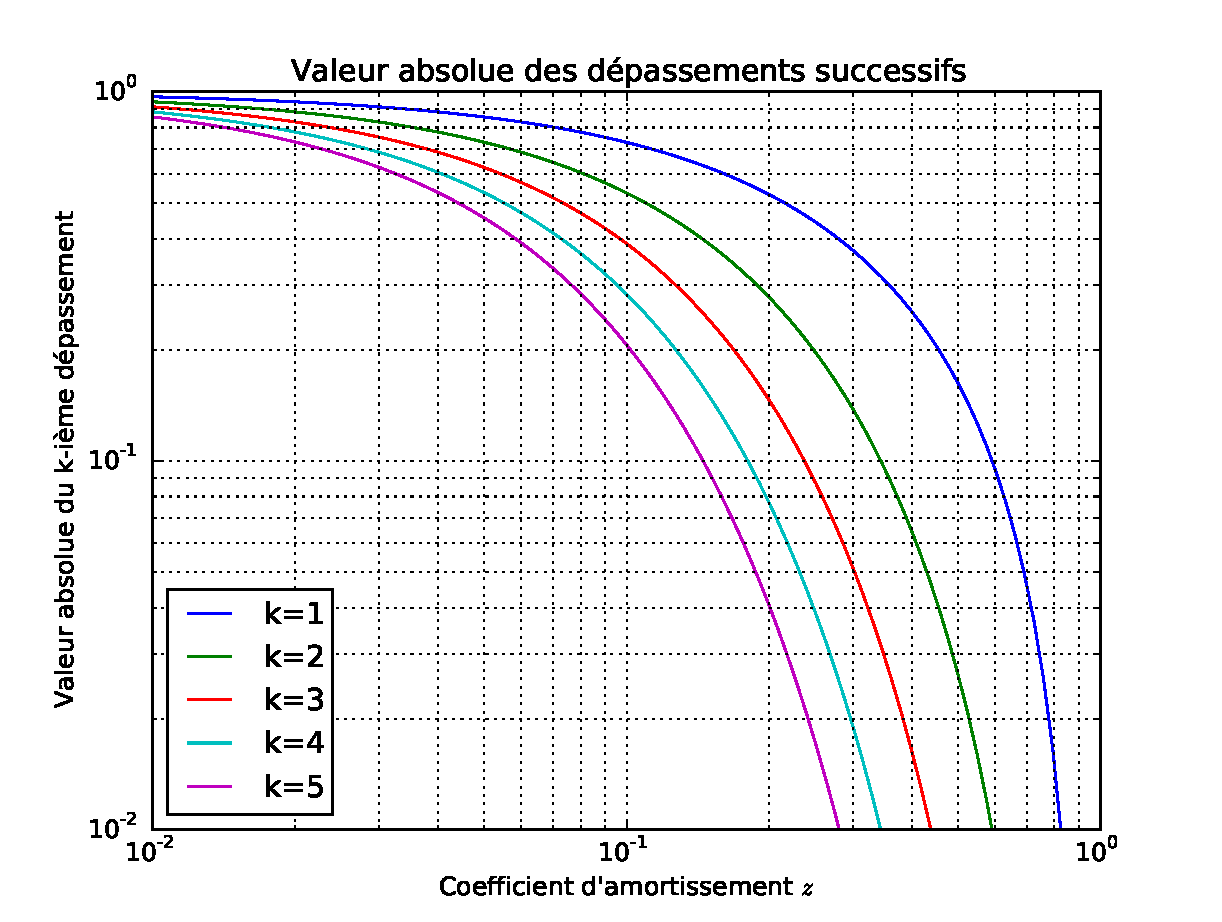
\includegraphics[width=\textwidth]{d5}
    \caption{Abaques des dépassements}
    \label{fig:abaque_dep}
\end{subfigure}
        
\caption{Abaques pour des systèmes d'ordre 2}
\label{fig:abaque}
\end{figure}

%
%
%\begin{resultat}
%\begin{center}
%\begin{tabular}{p{.4\linewidth}p{.58\linewidth}}
%\begin{center}
%\textbf{$\xi \geq 1$ : système non oscillant et amorti}
%
%\textbf{(apériodique)}
%
%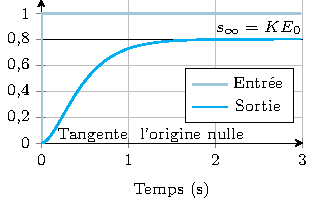
\includegraphics{Ordre2_amorti}
%\end{center} 
%& 
%\begin{center}
%\textbf{$\xi <1$ : système oscillant et amorti }
%
%\textbf{(pseudo périodique)}
%
%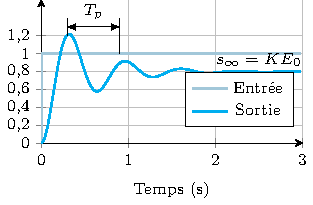
\includegraphics{Ordre2_pseudo}
%\end{center} 
%\begin{itemize} 
%\item La fonction de transfert a deux pôles réels.
%\item La tangente à l'origine est nulle.
%\end{itemize}
%& 
%\begin{itemize} 
%\item La fonction de transfert a deux pôles complexes.
%\item La tangente à l'origine est nulle.
%\item La pseudo-période est de la forme $T_p=\dfrac{2\pi }{\omega_0 \sqrt{1-\xi^2}}$.
%\item La valeur du premier dépassement vaut :  $D_1=KE_0e^{\dfrac{-\pi \xi }{\sqrt{1-\xi^2}}}$.
%\end{itemize}
%\end{tabular}
%\end{center}
%\end{resultat}
%
%\begin{resultat}
%\begin{itemize}
%\item Pour $\xi=0$ le système n'est pas amorti (oscillateur harmonique) la réponse à un échelon est une sinusoïde d'amplitude $KE_0$ ($2KE_0$ crête à crête).  
%\item Pour $\xi\simeq 0,69$  on obtient le système du second ordre le plus rapide \textbf{avec dépassement}. 
%Le temps de réponse à 5\% est donné par $t_{r 5\%} \cdot \omega_0 \simeq 3$.
%\item Pour $\xi =1$ on obtient le système du second ordre le plus rapide \textbf{sans dépassement}.
%
%\end{itemize}
%\end{resultat}
%
